\section{Deployment View}
This section shows the physical distribution of the system, that is, the environment in which the system runs. Specifically, \textit{Figure 2.4} shows the structure of the hardware components that execute the software.

Firewalls are inserted to ensure security between the different zones and load balancers are designed to distribute the workload.\\

As previously mentioned, the system is divided into 4 Tier, the components of which are described below:
\begin{itemize}
    \item \textbf{Client Tier}: it consists of the client programs used to exploit system services and the devices on which these programs are installed.
    \begin{itemize}
        \item \textbf{Smartphone}: users access the DREAM system and use the related services through a mobile application from a smartphone.
        \item \textbf{Personal Computer}: users access the DREAM system and use the related services through the Web browser from a personal computer.
    \end{itemize}
    \item \textbf{Web Tier}: it consists of components that handle the interaction between client tier and the business tier.  It contains the Web Server.
    \begin{itemize}
        \item \textbf{Web Server}: it provides content to the Web using the HTTP(S) protocol. It mainly works to serve the requested web pages continuously and without interruption. As long as the Web Server is up and running, the corresponding web pages and sites will be available to users on the network.
    \end{itemize}
    \item \textbf{Business Tier}: it processes all dynamic content and the interactions between the Client/Web Tier and the Data tier. It contains the Application Server.
    \begin{itemize}
        \item \textbf{Application Server}: it hosts and exposes business logic and processes. It provides the infrastructure and logical capabilities to support, develop and run applications in a distributed context. The Application Server communicates directly with the Mobile Application through HTTPS protocol, in order to create a lightweight API to request only the necessary data. The Application Server will receive this call, make the call to the external service, filter it, and return only what the application has requested.  This will reduce the amount of data transiting over mobile Internet and thus increase application performance.
    \end{itemize}
    \item \textbf{Data Tier}: it runs the DBMS and holds all of the sensitive application data. It contains database servers.
    \begin{itemize}
        \item \textbf{Database Server}: it allows access to one or more Database Systems and is an essential support for Web Servers in managing the delivery and storage of data. It communicates with the Application Server via the standard TCP/IP protocol and provides access to the physical database which is in charge of storing all persistent data of users who use DREAM.
    \end{itemize}
\end{itemize}\\


\textbf{Firewalls} are also included in the system architecture to delimit safe areas within the system. 
Specifically, there are firewalls between the Internet accessed by the customer to use the application and the Web Server and between the latter and the Application Server in order to create a demilitarized zone (DMZ). The purpose of the DMZ is to add an additional level of security to an internal network, where a node belonging to an external network can only access the services made available, without putting at risk and compromising the security of the entire network.
In order to ensure secure access to the database and to delimit the internal network (IN), a firewall is placed between the Application Server and the Database Server.\\


In order to distribute the load of the requests to the DREAM website among several servers, \textbf{load balancers} are introduced for the Web Server. In this way, the reliability and scalability of the entire architecture increases because requests will be shared equally among the different servers. If one of the servers is unable to respond to the request, the user can still use the service based on one of the active servers.
Similarly, the Web Server may need to query the database to generate responses. Web Servers send database queries to the load balancer which balances the inbound database workload on the database servers.



\def\fillandplacepagenumber{%
 \par\pagestyle{empty}%
\vbox to 0pt{\vss}\vfill
\vbox to 0pt{\baselineskip0pt
   \hbox to\linewidth{\hss}%
   \setlength{\footskip}{70pt}
   \baselineskip\footskip
   \hbox to\linewidth{%
     \hfil\thepage\hfil}\vss}}

\begin{landscape}
\begin{figure}[h]
\vspace*{-2cm}
\noindent
\centering
\centerline{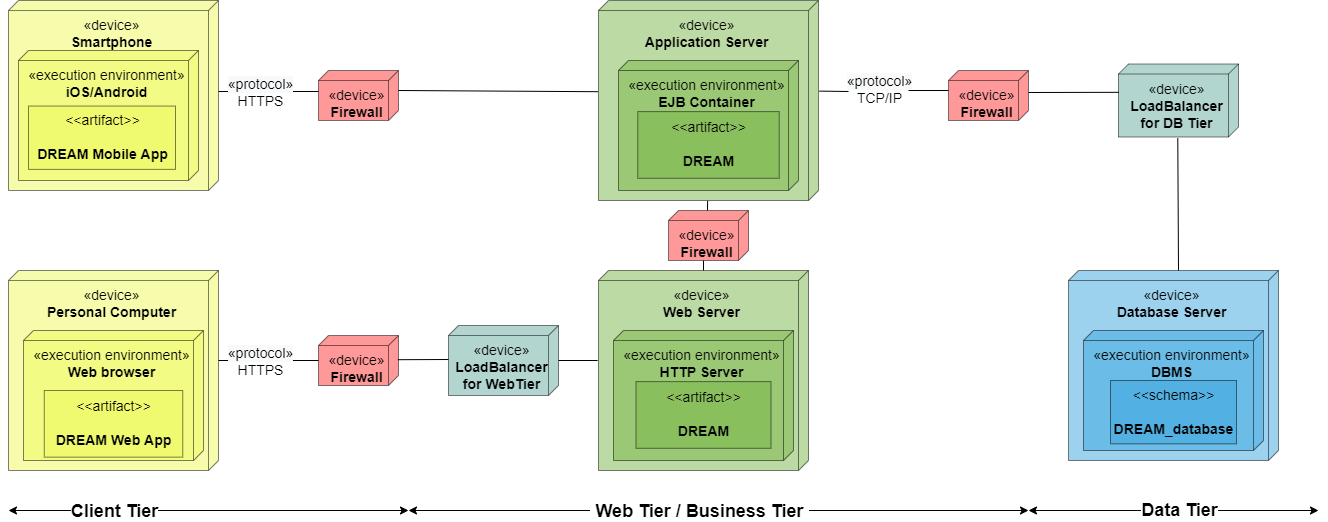
\includegraphics[scale = 0.6]{./Images/Deployment diagram.png}}
    \caption{Deployment diagram}
    \vspace*{-12cm}
\end{figure}
\fillandplacepagenumber
\end{landscape}



